The complete pipeline starting from capturing the video of the laser sweeping
across an object to the end result of visualizing the 3D model of
reconstructed point cloud is primarily divided into five major steps as shown
in figure \ref{figure:pipeline}.

\begin{figure}[ht!]
\centering
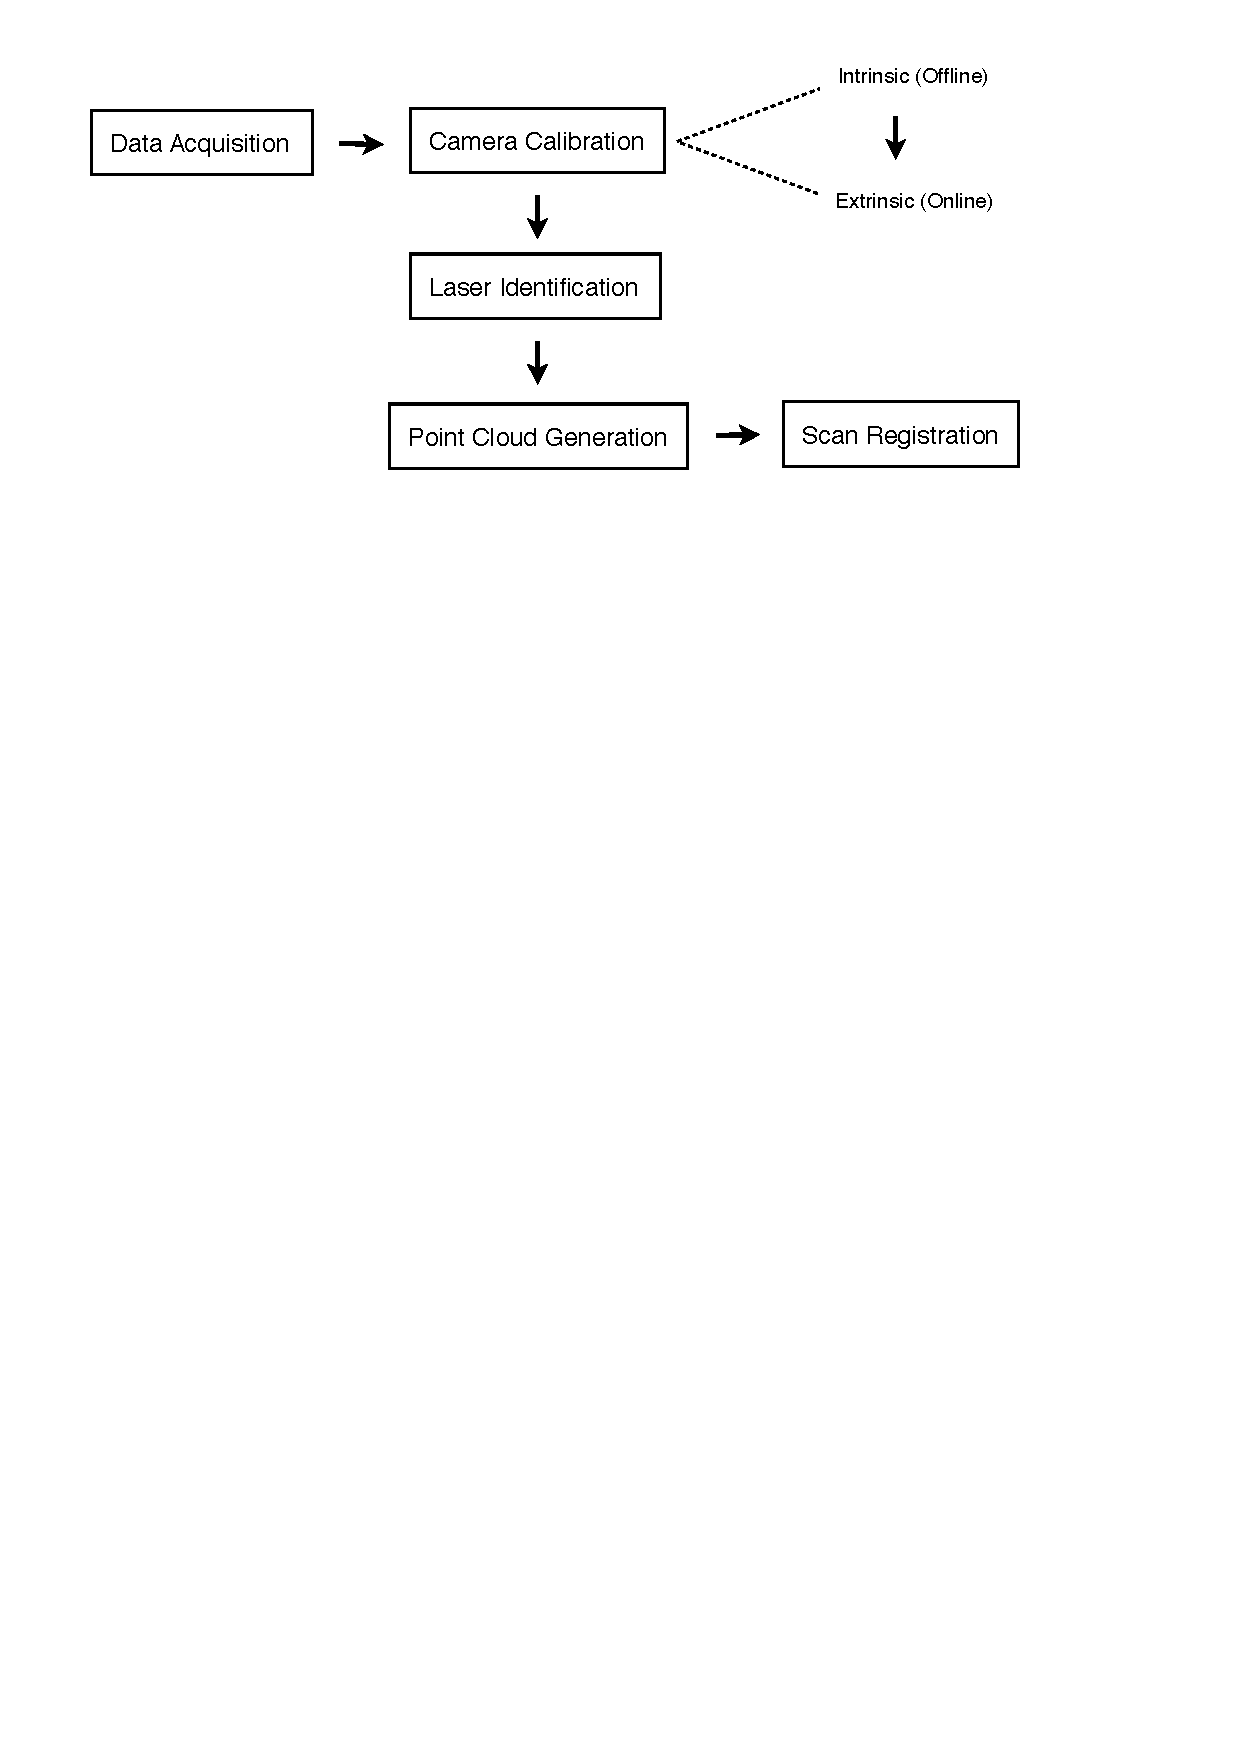
\includegraphics[width=1.0\linewidth]{figures/pipeline}
\caption{Software Pipeline}
\label{figure:pipeline}
\end{figure}

\subsection{Data Acquisition}
\label{subsection:data-acquistion}
\begin{figure}[ht!]
\centering
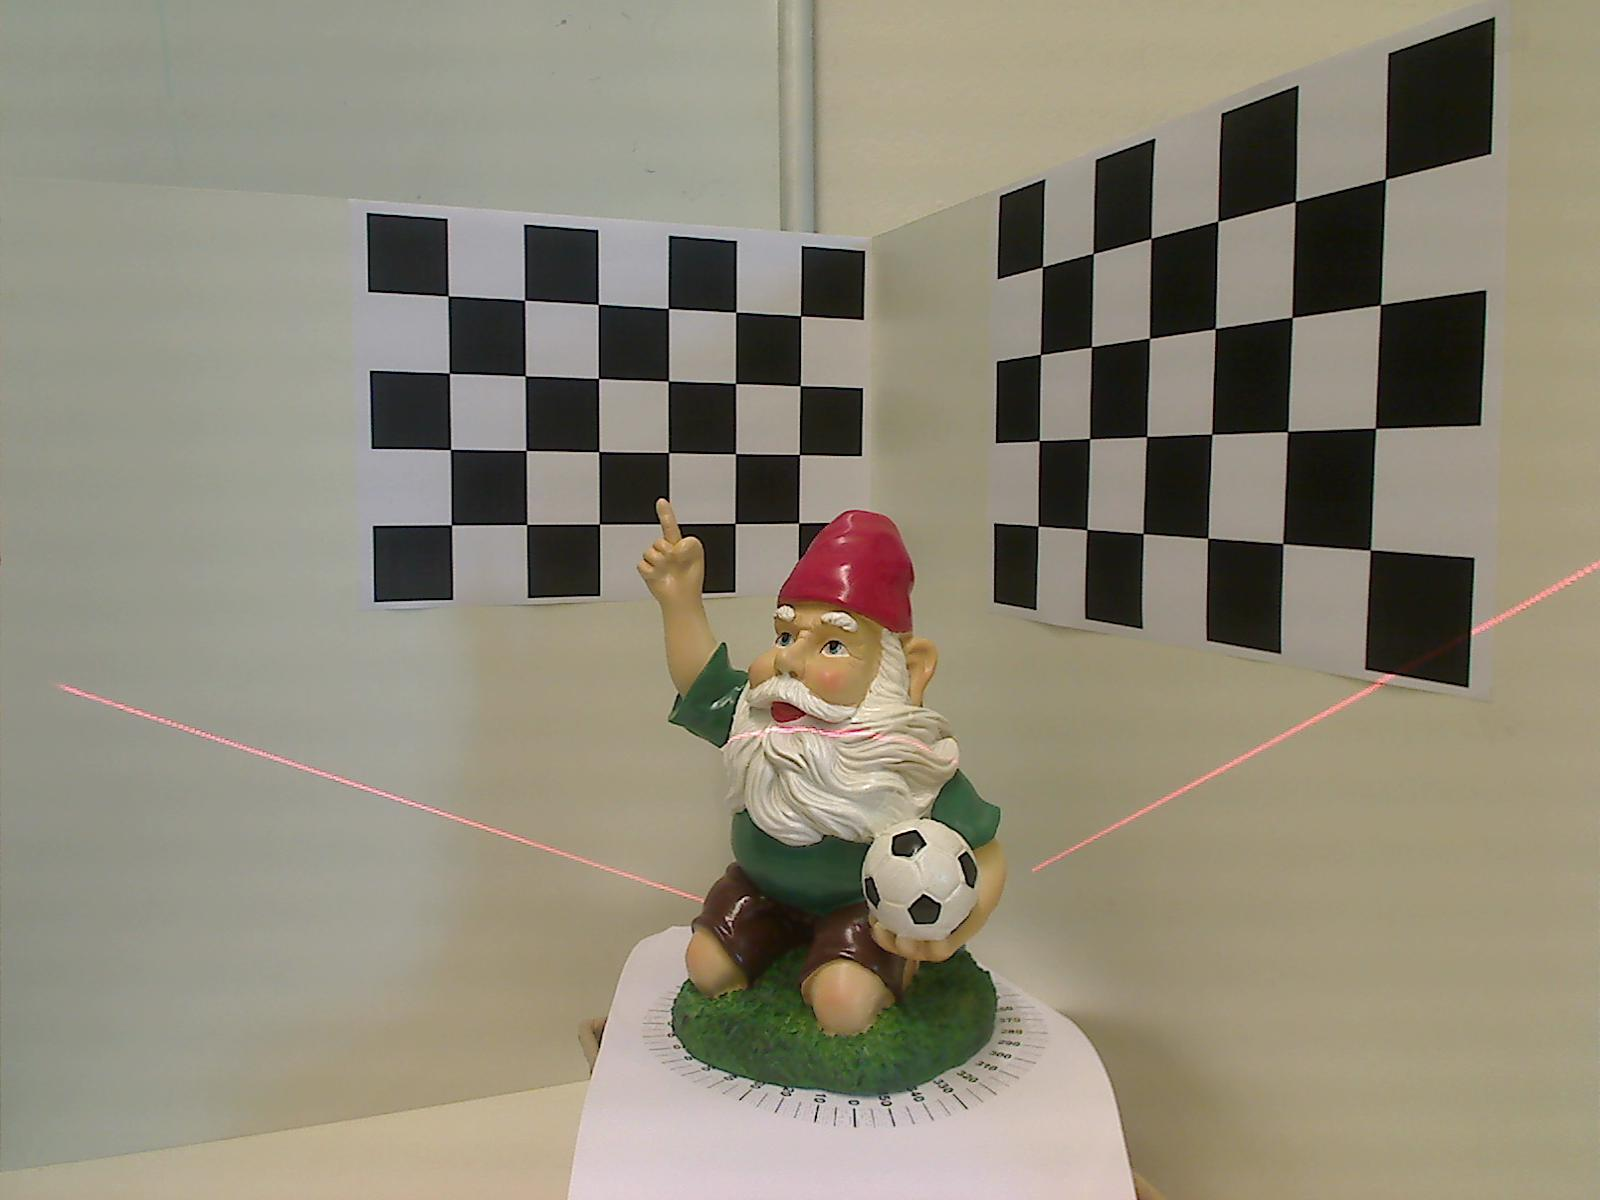
\includegraphics[width=0.5\linewidth]{figures/introduction}
\label{figure:acquisition}
\caption{Data Acquisition}
\end{figure}

We used a standard digital camera to capture multiple runs of a hand-held laser sweeping across the object as shown in figure \ref{figure:acquisition}. Since the videos were stored in raw format which cannot be directly processed by OpenCV, we used \texttt{mplayer} to extract individual frames at the rate of 5 frames per second.

\begin{verbatim}
$ mplayer -demuxer rawvideo \
          -rawvideo fps=5:w=1600:h=1200:yuy2 \
          -vo pnm:ppm $FILE	
\end{verbatim}

These frames were then later read into memory by calling the OpenCV routine \texttt{cvLoadImage()} with a \texttt{CV\_LOAD\_IMAGE\_UNCHANGED} flag. The routine allocates an image data structure and returns a pointer to a struct of type \texttt{IplImage}



\subsection{Camera Calibration}
\label{subsection:camera-calibration}
The first step in the process of reconstructing the 3D geometry of the object
is to establish a mathematical relationship between the natural units of the
camera with the physical units of the 3D world. We use camera calibration to
estimate the internal parameters of the camera and its distortion coefficients.
The geometry is described in terms of camera's optical center and focal
length of the camera.

\begin{figure}[ht!]
\centering
\subfigure{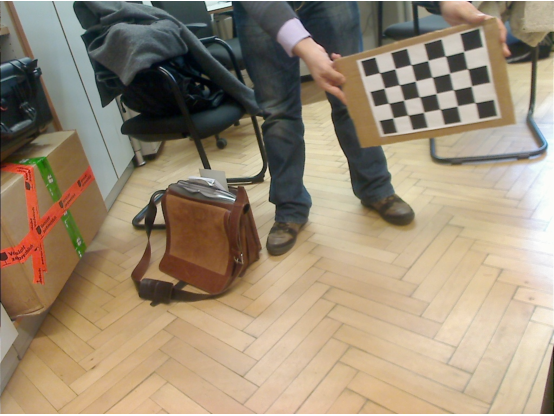
\includegraphics[width=.48\linewidth]{figures/calibrate-1}}\quad
\subfigure{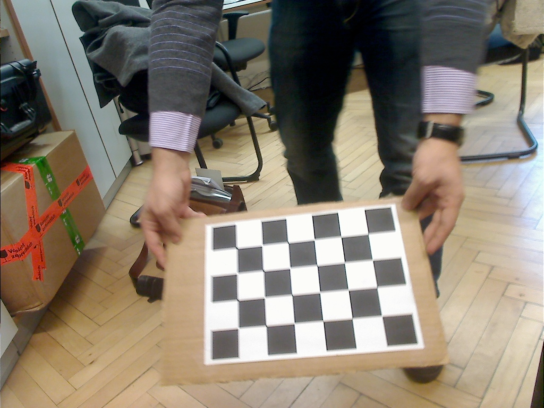
\includegraphics[width=.48\linewidth]{figures/calibrate-2}} \\
\subfigure{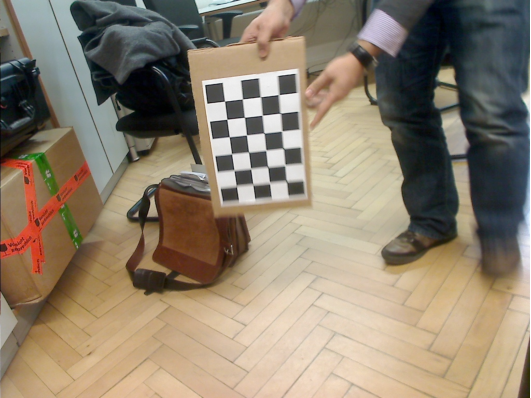
\includegraphics[width=.48\linewidth]{figures/calibrate-3}}\quad
\subfigure{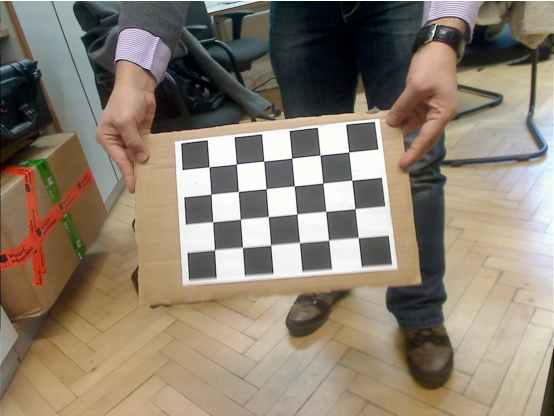
\includegraphics[width=.48\linewidth]{figures/calibrate-4}}
\caption{Calculating the Camera's Intrinsic Parameters}
\label{figure:camera-calibration-intrinsics}
\end{figure}

We use OpenCV camera calibration routines and a planar chessboard pattern as
our calibration object. OpenCV uses Zhang's method \cite{zhang:2000} to
calculate the focal lengths and offsets. However it uses Brown's method
\cite{brown:1971} to calculate the distortion coefficients. The calibration
pattern is rotated and translated to provide multiple views in order to get
precise information about the intrinsic parameters of the camera as shown in
Fig.  \ref{figure:camera-calibration-intrinsics}.  The OpenCV routine
\texttt{cvFindChessboardCorners()} is used to locate the corners and once we
have enough corners from multiple images, we use \texttt{cvCalibrateCamera2()}
to get the intrinsic matrix $A$ as shown in Eq. \ref{equation:calibrate}.

\begin{align}
	\label{equation:calibrate}
	s \times
	\begin{bmatrix}
		u \\ v \\	1 \\
	\end{bmatrix} &= A \cdot \begin{bmatrix}
															R \mid T
	 				  								\end{bmatrix}
										 \cdot \begin{bmatrix}
															x_w \\ y_w \\ z_w \\ 1
														\end{bmatrix} \\
	\text{where}~
	A &= \begin{bmatrix}
					f_x & 0 & c_x \\
					0 & f_y & c_y \\
					0 & 0 & 1 \\
 		 	 \end{bmatrix} \notag
\end{align}

The intrinsic matrix $A$ is later used to describe the pose of the object
being scanned by the laser relative to the coordinate system of the camera. In
order to determine this pose on both sides of the target object, the patterns
are masked to allow individual calculation as shown in Fig.
\ref{figure:camera-calibration-extrinsics}. The parameters represented by
$\begin{bmatrix}R \mid T\end{bmatrix}$ are then separately calculated for both
the sides by calling the OpenCV routine
\texttt{cvFindExtrinsicCameraParams2()}.

\begin{figure}[ht!]
\centering
\subfigure[$R_1 \mid T_1$]
{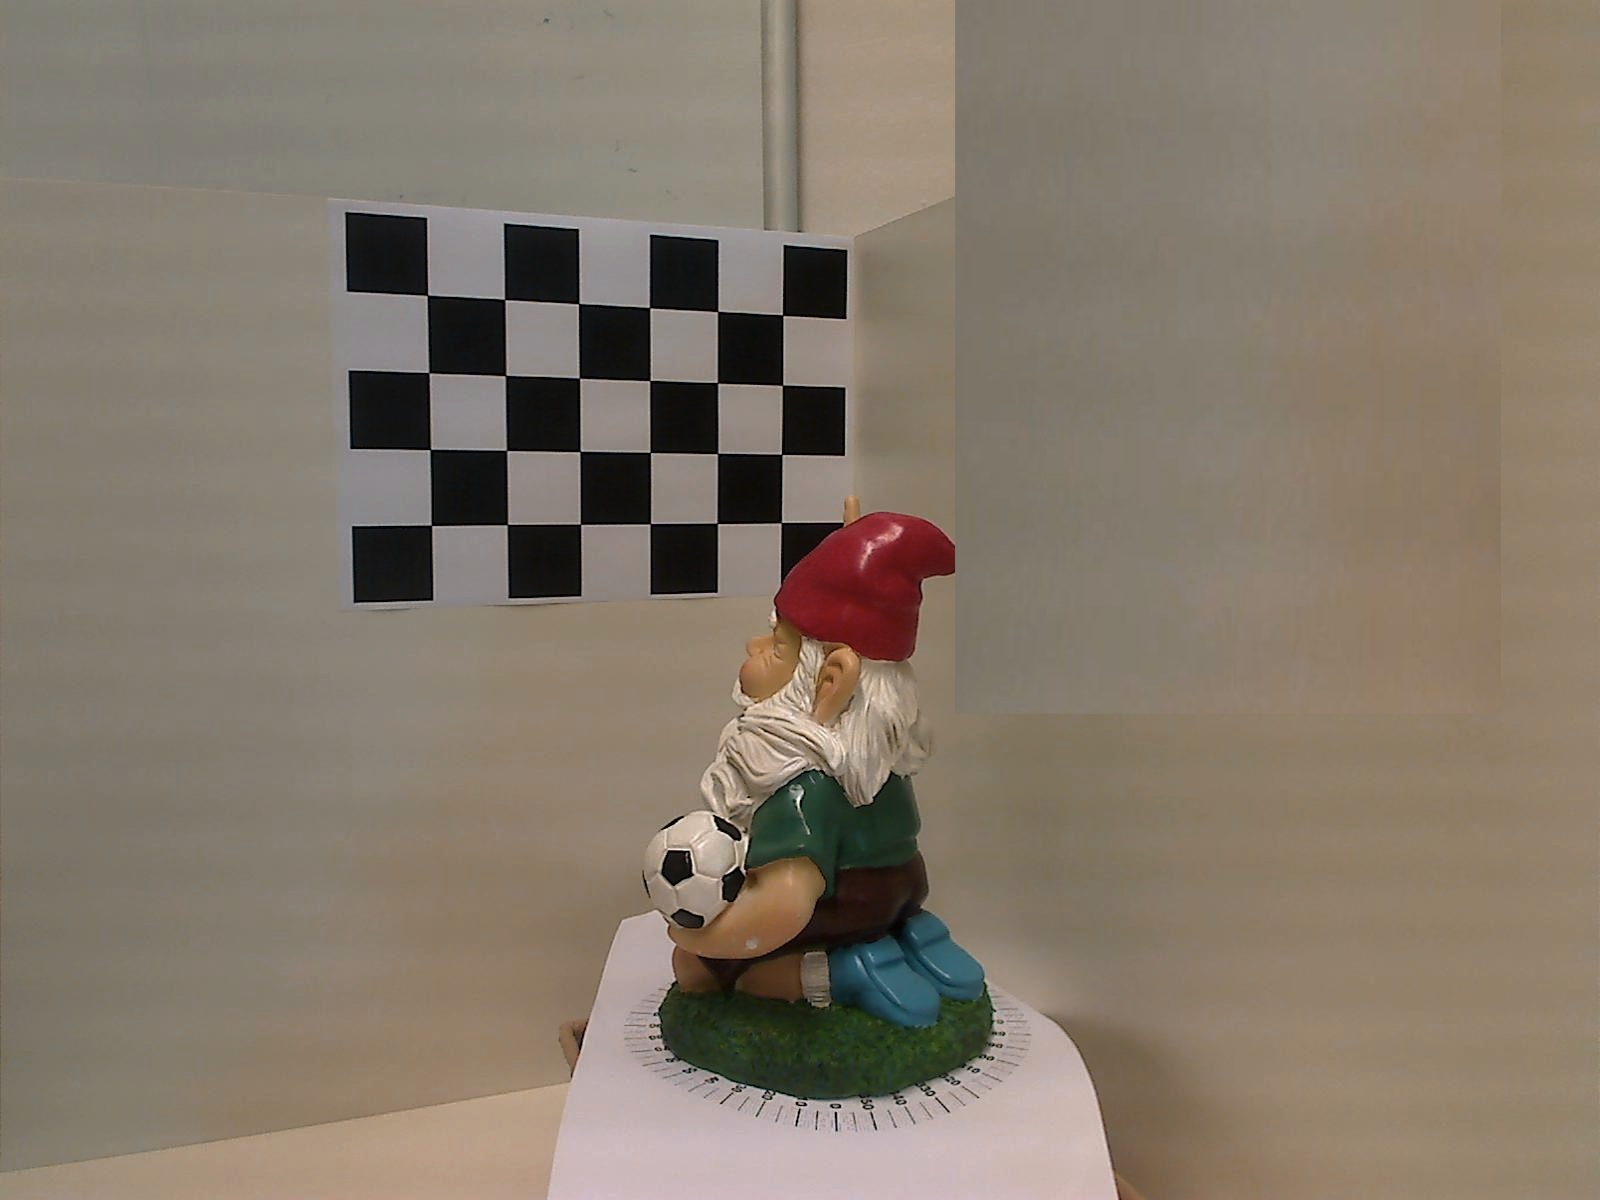
\includegraphics[width=.47\linewidth]{figures/calibrate-5}} \quad
\subfigure[$R_2 \mid T_2$]
{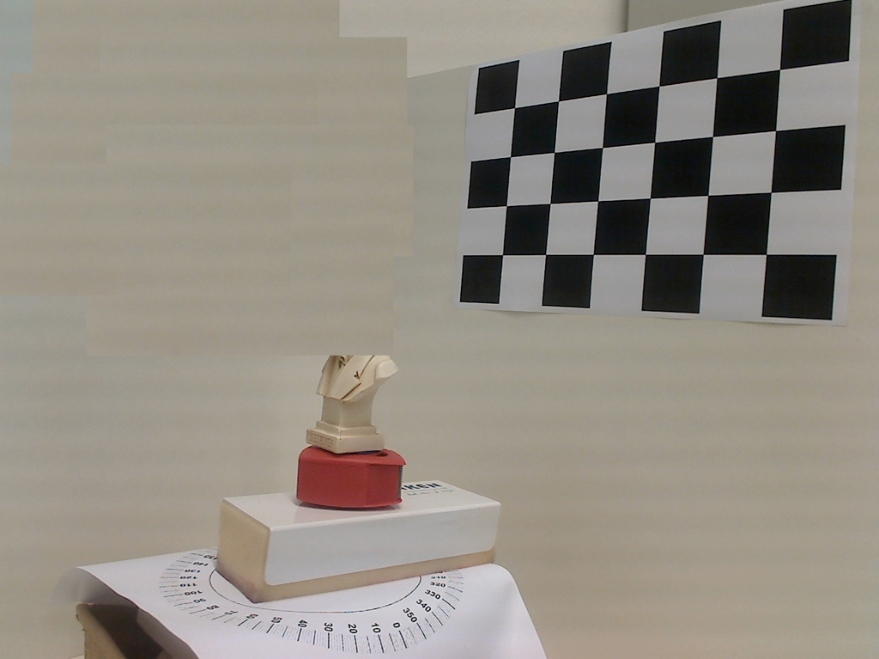
\includegraphics[width=.47\linewidth]{figures/calibrate-6}}
\caption{Calculating the Camera's Extrinsic Parameters}
\label{figure:camera-calibration-extrinsics}
\end{figure}



\subsection{Identification of 2D Laser Lines and Object Points}
\label{subsection:search-laser}
\begin{figure}[ht!]
\centering
\subfigure[$X$]
{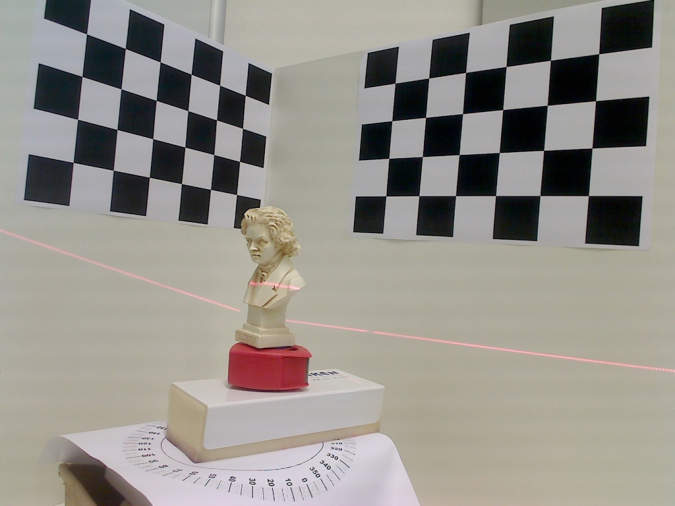
\includegraphics[width=.48\linewidth]{figures/difference-1}
 \label{subfigure:diff-A}} \hfill
\subfigure[$Y$]
{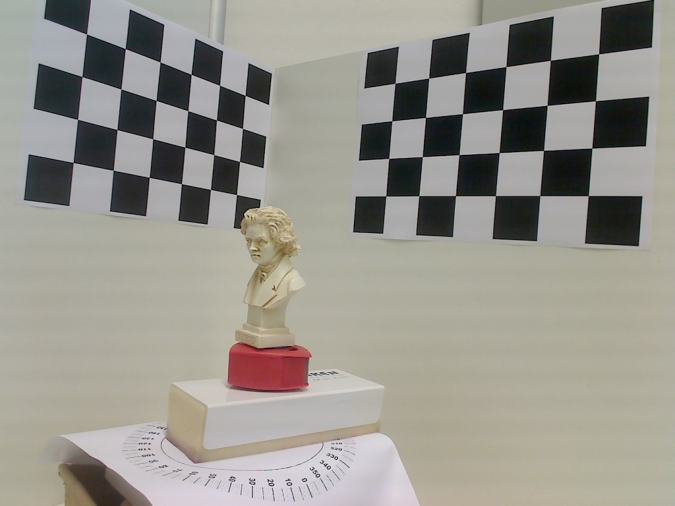
\includegraphics[width=.48\linewidth]{figures/difference-2}
\label{subfigure:diff-B}} \\
\subfigure[$Z$]
{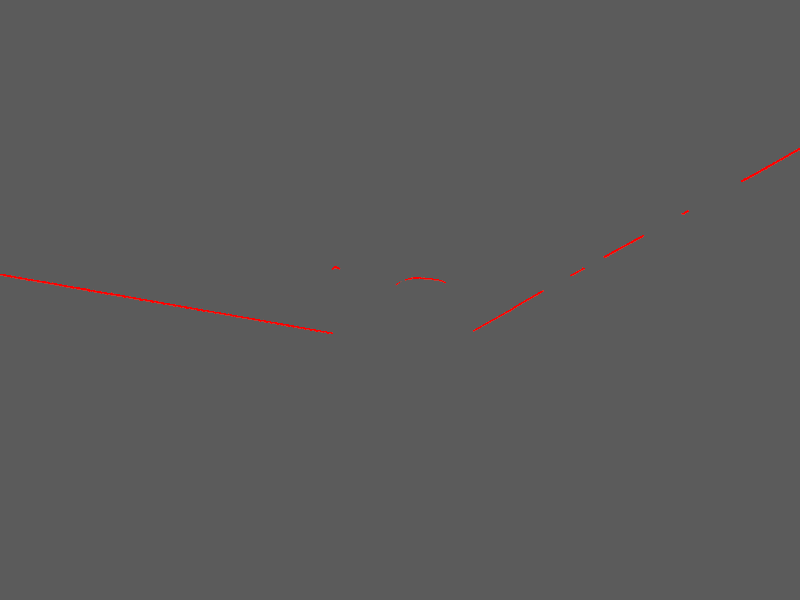
\includegraphics[width=.48\linewidth]{figures/colorthres}
\label{subfigure:diff-C}} \hfill
\caption{Using Image Difference to Find the Laser}
\label{figure:difference-image}
\end{figure}

We use OpenCV routine \texttt{cvAbsDiff()} to calculate the image difference
of the laser image from the reference image using Eq.
\ref{equation:difference-image}. The resulted image difference is shown in
Fig. \ref{figure:difference-image}

\begin{align}
\label{equation:difference-image}
Z = X &- Y \\
\text{where}~
&X~ \text{is the laser image in figure \ref{subfigure:diff-A} and} \notag \\
&Y~ \text{is the reference image in figure \ref{subfigure:diff-B} and} \notag \\
&Z~ \text{is the difference image in figure \ref{subfigure:diff-C}} \notag
\end{align}

To reduce the noise in the difference image, we use the OpenCV routine
\texttt{cvSmooth()} to convolve the image with a Gaussian kernel function. It
not only helps to remove the camera artifacts but also reduces the information
content in the image. In order to remove all outliers and keep just the pixels
representing the red laser line, we use a pre-defined threshold value for the
intensity of the red pixels. In order to restrict this thresholding only along
the red channel, we use \texttt{cvSplit()} to split the three-channel (R,G,B)
difference image into separate one-channel image planes. We use
\texttt{cvGet2D()} and \texttt{cvSet2D()} to work on the scalar values of the
pixels.

%\begin{figure}[ht!]
%\centering
%\subfigure[Image with Outliers]
%{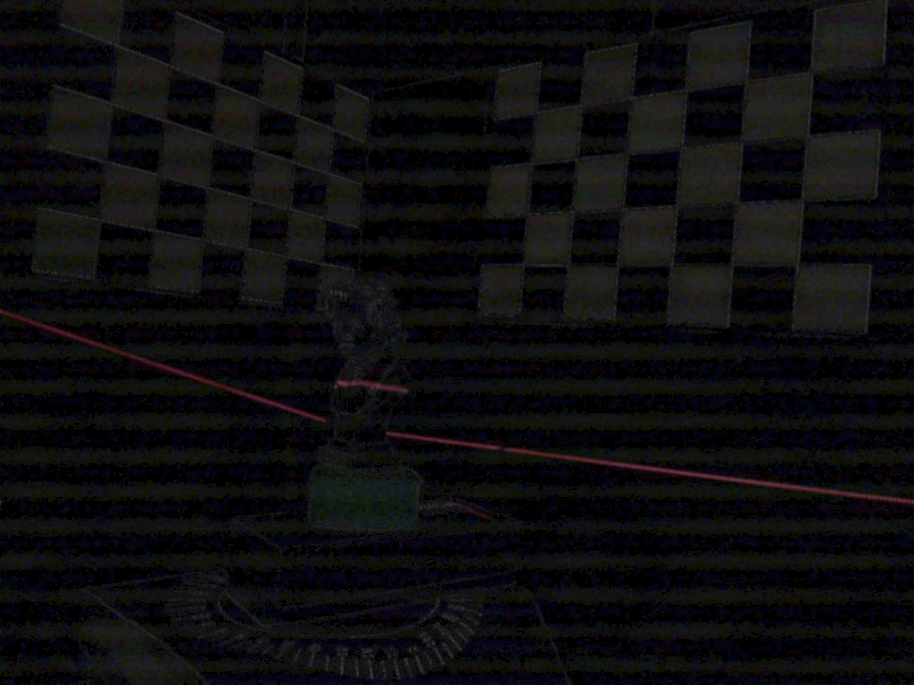
\includegraphics[width=.45\linewidth]{figures/gauss}
%\label{subfigure:colorthres-A}} \quad
%\subfigure[Image without Outliers]
%{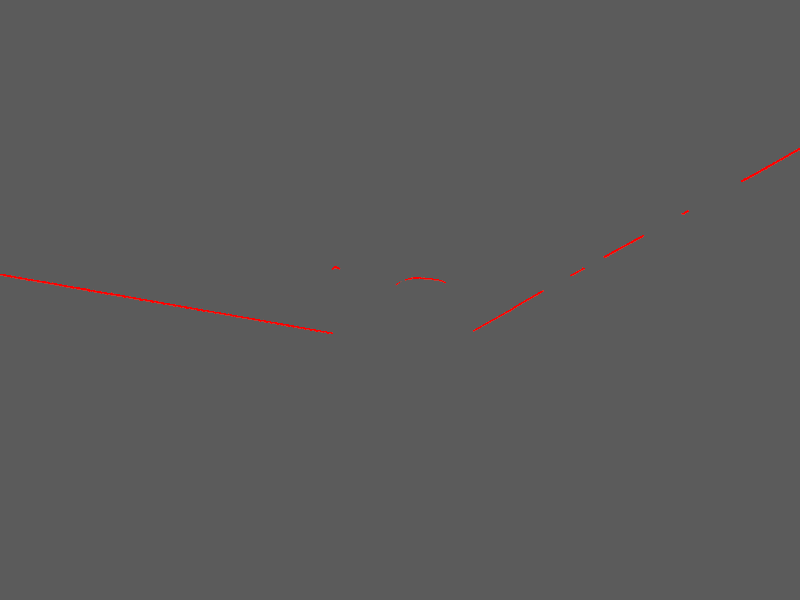
\includegraphics[width=.45\linewidth]{figures/colorthres}
%\label{subfigure:colorthres-B}} \hfill
%\caption{Color Thresholding to Remove Outliers}
%\label{figure:color-thres}
%\end{figure}

%\begin{figure}[ht!]
%\centering
%\subfigure[Image with Outliers]
%{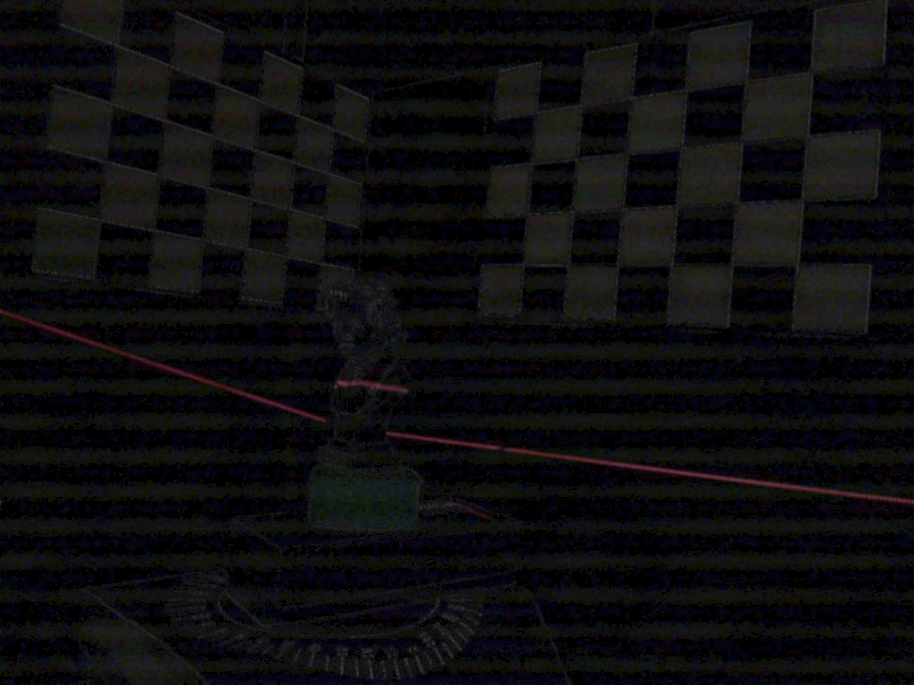
\includegraphics[width=.45\linewidth]{figures/gauss}
%\label{subfigure:colorthres-A}} \quad
%\subfigure[Image without Outliers]
%{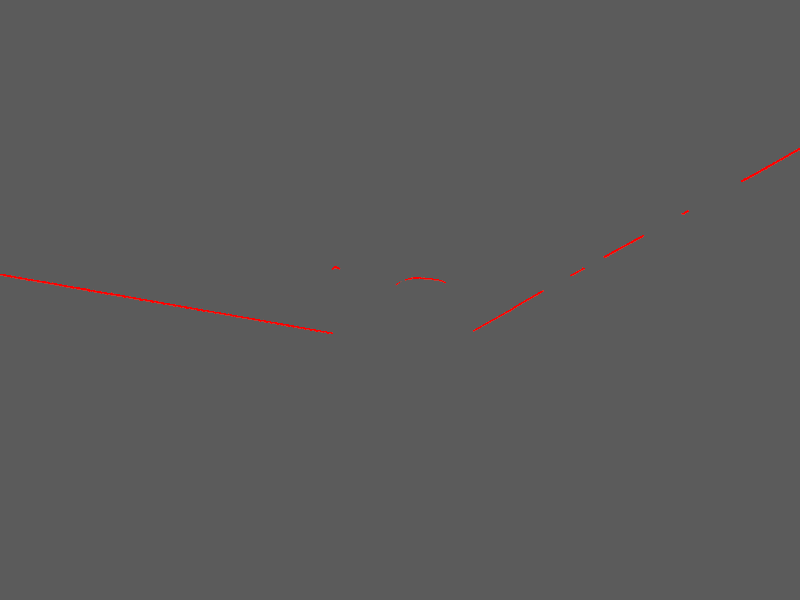
\includegraphics[width=.45\linewidth]{figures/colorthres}
%\label{subfigure:colorthres-B}} \hfill
%\caption{Color Thresholding to Remove Outliers}
%\label{figure:color-thres}
%\end{figure}

We use the \ac{PPHT} \cite{kiryati:1991}, \cite{matas:2000} using the OpenCV
routine \texttt{cvHoughLines2()} to detect the laser lines on both sides of
the target object. The line end points of each line thus obtained are used to
draw the line using \texttt{cvLine()} as shown in Fig.
\ref{figure:hough-transform}.  The difference image is initially passed
through an edge detection phase, since the hough transform not only expects a
gray-scale image as input but the input is also treated as binary information
where the non-zero points are edge points of the image. Therefore, we use the
OpenCV routine \texttt{cvCvtColor} to convert the RGB difference image to gray
scale and \texttt{cvCanny()} to perform the Canny Edge Detection
\cite{canny:1986} before \ac{PPHT}. The two hough line equations on either
side of the object are used to find the laser line points, while the points
not identified as part of the hough line are taken as target object points.

\begin{figure}[ht!]
\centering
\subfigure[Before Transformation]
{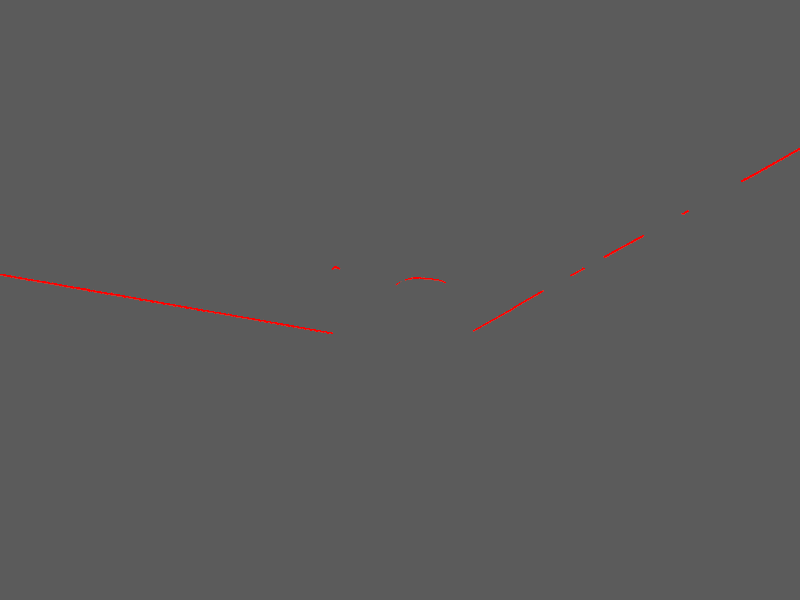
\includegraphics[width=.46\linewidth]{figures/colorthres}
\label{subfigure:hough-A}} \quad
\subfigure[After Transformation]
{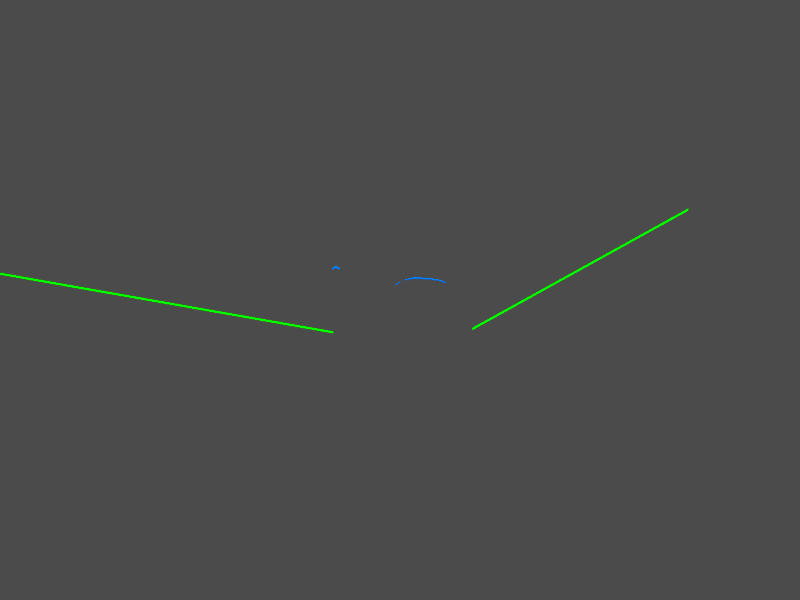
\includegraphics[width=.46\linewidth]{figures/hough}
\label{subfigure:hough-B}} \\
\caption{Hough Transformation}
\label{figure:hough-transform}
\end{figure}


\subsection{Generation of Point Cloud}
\label{subsection:generate-pointcloud}
\begin{figure}[ht!]
\centering
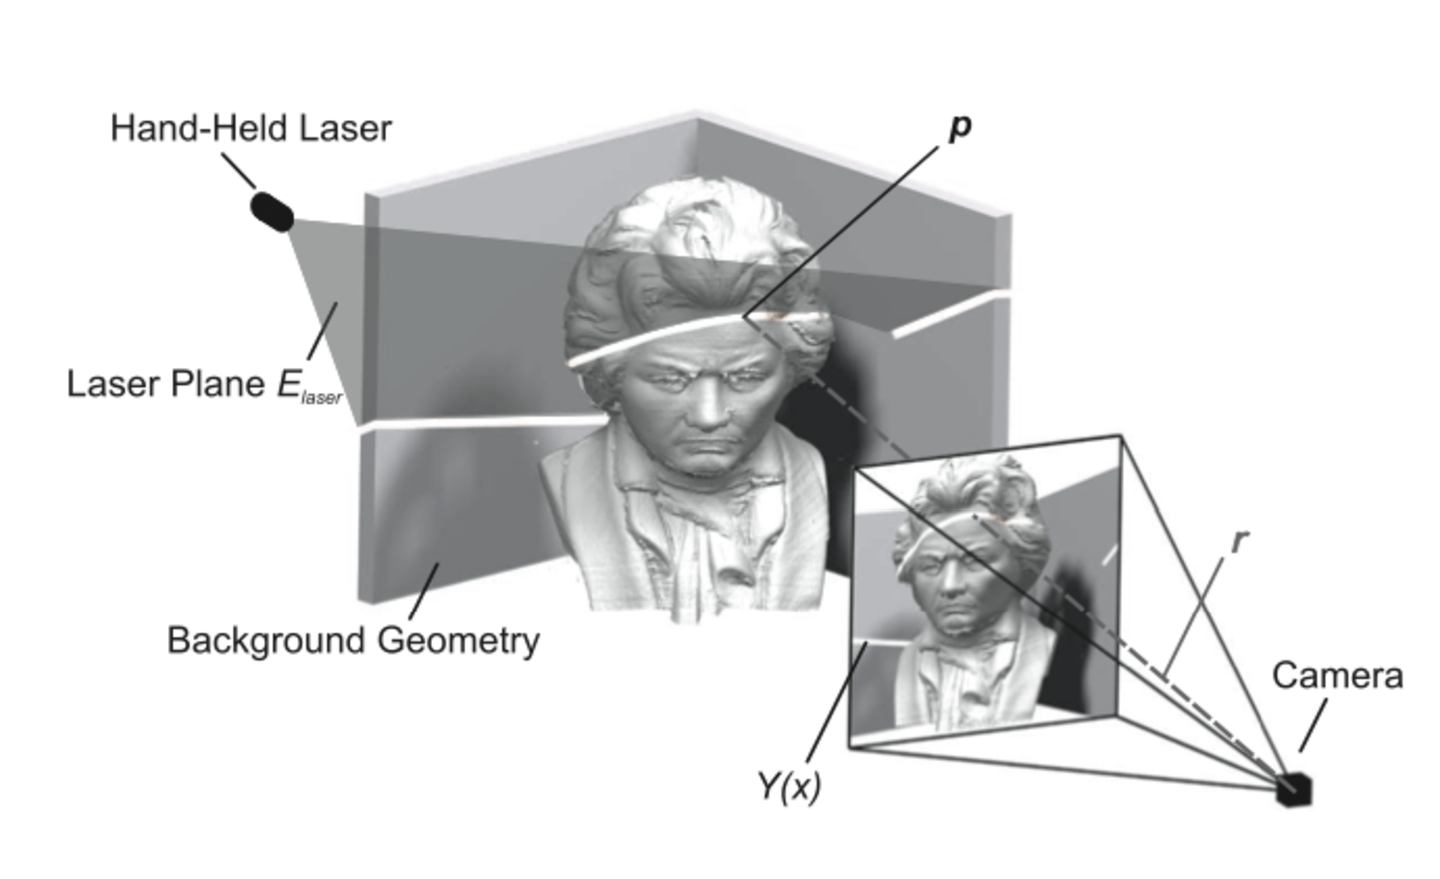
\includegraphics[width=1.0\linewidth]{figures/pointcloudpaper}
\caption{Laser Triangulation \cite{winkelbach:2006}}
\label{figure:triangulation}
\end{figure}

The first step is to use the calculated camera extrinsics ($R \mid T$) for
each side of the target object along with the intrinsic parameters ($A$) to
transform each laser pixel ($P_c$) into 3D laser surface points ($P_w$) using
Eq. \ref{equation:3dlaserpoint}. The laser pixel points are expressed in
the homogenous coordinate system.

\begin{align}
	\label{equation:3dlaserpoint}
	P_w &= 	\underbrace{s \cdot R^{-1}
 					 							\cdot A^{-1}
 												\cdot P_c
										 }_\text{$\overrightarrow{b}$}
					-
					\underbrace{
											R^{-1} \cdot T
										 }_\text{$\overrightarrow{a}$} \\
	\text{where}~
	P_c &= \begin{pmatrix}
						u \\
						v \\
						1 \\
				 \end{pmatrix},
	\overrightarrow{a} = \begin{pmatrix}
													a_x \\
													a_y \\
													a_z \\
												\end{pmatrix},
	\overrightarrow{b} = \begin{pmatrix}
													b_x \\
													b_y \\
													b_z \\
												\end{pmatrix} \notag \\
  \text{and}~ s &= \frac{a_z}{b_z} \notag
\end{align}

Next, in order to bring all the laser surface points into a common coordinate
system, we transform all the 3D laser points from the right side of the
target object to the coordinate system of the left side using Eq.
\ref{equation:right2left}

\begin{align}
	\label{equation:right2left}
	P_{l} &= R_1^{-1} \times P_{r} - R_1^{-1}T_1 \\
	\text{where}~
	P_{r} &= \begin{bmatrix}
									R_2 \mid T_2
 				  \end{bmatrix} \times P_w \notag
\end{align}

With all the 3D laser surface points in a common coordinate system, we
randomly choose 3 points to generate the laser plane equation. Using the
coefficients of this equation, we define the normal to the plane
$(\overrightarrow{N})$ using Eq. \ref{equation:laserplaneequation}.

\begin{align}
	\label{equation:laserplaneequation}
	E_x + F_y + G_z + H &= 0 \\
	\text{where}~
	 \overrightarrow{N} &=
	 \begin{pmatrix}
	  E \\
	  F \\
	  G \\
	 \end{pmatrix} \notag
\end{align}

The last step is to use the target object pixels $(P_c)$ and intersect them
with the laser plane equation represented by the normal $(\overrightarrow{N})$
to obtain the 3D surface points of the target object $(P_w)$ as shown in
Fig. \ref{figure:triangulation} using Eq. \ref{equation:3dobjectpoint}

\begin{align}
	\label{equation:3dobjectpoint}
	P_w &= s \times R^{-1}
 					 \times A^{-1}
					 \times P_c
					- R^{-1} \times T \\
	\text{where}~
	s &= \frac{\overrightarrow{N}\times\overrightarrow{a} - D}
						{\overrightarrow{b}\times\overrightarrow{N}}
  ~\text{and}~ P_c = \begin{pmatrix}
												u \\
												v \\
												1 \\
										 \end{pmatrix} \notag
\end{align}

We also use the OpenCV routine \texttt{cvGet2D()} to retrieve the RGB color
information for each object pixel and map it to the calculated corresponding
3D object surface point. We use the reference image as the source for
retrieving the original color information since that image does not have a
laser line sweeping the target object.


\subsection{Point Cloud Processing and Registration}
\label{subsection:registration}
\begin{itemize}
	\item 3DTK
\end{itemize}
